\documentclass[12 pt]{article}
\usepackage{amssymb}
\usepackage{amsmath}
\usepackage{amsthm}
\usepackage{amsfonts}
\usepackage{fullpage}
\usepackage[mathscr]{euscript}
\usepackage{youngtab}
\usepackage{graphicx}
\usepackage{color}
\usepackage{multirow}
\usepackage{enumerate}
\usepackage{listings}
\newcommand{\W}{\mathcal{W}}
\newcommand{\C}{\mathbb{C}}
\newcommand{\R}{\mathbb{R}}
\newcommand{\Z}{\mathbb{Z}}
\newcommand{\N}{\mathcal{N}}
\newcommand{\M}{\mathcal{M}}
\newcommand{\OO}{\mathcal{O}}
\newcommand{\B}{\mathcal{B}}
\newcommand{\pf}{\tilde{\phi}_N}
\newcommand{\g}{\mathfrak{g}}
\newcommand{\su}{\mathfrak{su}}
\newcommand{\so}{\mathfrak{so}}
\newcommand{\usp}{\mathfrak{usp}}
\newcommand{\h}{\mathfrak{h}}
\newcommand{\BB}{\mathfrak{B}}
\newcommand{\mon}{\OO_{\vec{n}}(a)}
\newcommand{\I}{\mathcal{I}}
\numberwithin{equation}{section}
\begin{document}

\title{Boston Housing Prices \\ \footnotesize{Udacity Machine Learning Engineer \\ Nanodegree Program: Project 1}}
\author{Anderson Daniel Trimm}
\date{\today}
\maketitle
\begin{abstract}
In this report, we explore the Boston Housing dataset and train a decision tree regressor to predict housing prices.
\end{abstract}
\section{Introduction}
In this project, we use machine learning to make a predictive model of Boston housing prices in the 1970s using the Boston housing price data set. This is a (supervised) regression learning problem, and we model our data using scikit-learn's decision tree regressor. After exploring the data in section \ref{stats} by making a statistical analysis using NumPy, in section \ref{predict} we train our model, evaluate its performance on the training and testing data, and finally use it to predict the price of a new house. In section \ref{conclusions}, we discuss our conclusions.
\section{Statistical Analysis of the Boston Housing Dataset}\label{stats}
In this section we compute basic statistics of the Boston Housing dataset using NumPy. To begin, we need to import the Boston Housing dataset as well as Numpy:

\begin{verbatim}
	import numpy as np
	from sklearn import datasets
\end{verbatim}

We can now define the following function to load the Boston dataset:

\begin{verbatim}
	def load_data():
    """Load the Boston dataset."""

    boston = datasets.load_boston()
    return boston
\end{verbatim}
After loading the Boston dataset, we can look at its attributes \texttt{boston.data} and \texttt{boston.target} to access the features and housing prices. The attribute \texttt{boston.data} gives a two-dimensional ndarray, where each row is the list of features for a given house. The attribute \texttt{boston.target} gives a one-dimensional ndarray of the housing prices. The total number of houses is therefore just the length of the ndarray boston.target:

\begin{verbatim}
	>>> np.shape(boston.target)
(506,)
\end{verbatim}
which we see is 506. The number of features per house then is the row length of the ndarray boston.data, which is the one-eth entry of
\begin{verbatim}
	>>> np.shape(boston.data)
(506, 13)
\end{verbatim}
which is 13. We can encapsulate these in functions as 
\begin{verbatim}
		def size_of_data(city_data):
    number_of_houses = np.shape(city_data.data)[0]
    return number_of_houses
\end{verbatim}
\begin{verbatim}
	def number_of_features(city_data):
    number_of_features = np.shape(city_data.data)[1]
    return number_of_features
\end{verbatim}

To compute the minimum, maximum, mean, and meadian price, as well as the standard deviation, we simply use the methods \texttt{np.min(boston.target)},\texttt{np.max(boston.target)}, \texttt{np.mean(boston.target)}, \texttt{np.meadian(boston.target)}, and \texttt{np.std(boston.target)}, respectively. We find
\begin{verbatim}
	>>> np.min(boston.target)
5.0
>>> np.max(boston.target)
50.0
>>> np.mean(boston.target)
22.532806324110677
>>> np.median(boston.target)
21.199999999999999
>>> np.std(boston.target)
9.1880115452782025
\end{verbatim}
As before, we can encapsulate these in functions as
\begin{verbatim}
	def get_min_price(city_data):
    min_price = np.min(city_data.target)
    return min_price
\end{verbatim}
\begin{verbatim}
	def get_max_price(city_data):
    max_price = np.max(city_data.target)
    return max_price
\end{verbatim}
\begin{verbatim}
def get_mean_price(city_data):
    mean_price = np.mean(city_data.target)
    return mean_price
\end{verbatim}
\begin{verbatim}
	def get_median_price(city_data):
    median_price = np.median(city_data.target)
    return median_price
\end{verbatim}
\begin{verbatim}
	def get_standard_deviation(city_data):
    standard_deviation = np.std(city_data.target)
    return standard_deviation
\end{verbatim}

\section{Predicting Housing Prices}\label{predict}
In this section we will model the dataset using a decision tree regressor. After discussing our choice of performance metric, we train and cross-validate our model by performing a grid  search over possible max depths of our decision tree. We visualize our model's performance by plotting the learning curve for each max depth, and combine these into a model complexity graph. After determining the  optimal max depth for our decision tree, we use our model to predict the price of a new house, and compare with the statistics computed in section \ref{stats}.
\subsection{Evaluating Model Performance}
Since we would like to be able to evaluate our model's ability to predict housing prices given new, unseen data, we begin by splitting the Boston dataset into a training and testing set. By holding out the testing data and allowing our model to learn only on the training set, we leave ourselves an independent set of data we can use to verify that our model can generalize well to unseen data. If we trained on the \emph{entire} dataset, we would have no way to evaluate how well our model can predict the housing price of new data points.

To split the dataset, we first import \texttt{train\_test\_split} from the \texttt{sklearn.cross\_validation} module:
\begin{verbatim}
	from sklearn.cross_validation import train_test_split
\end{verbatim}
and define the function 
\begin{verbatim}
	def split_data(city_data):
    # Get the features and labels from the Boston housing data
    X, y = city_data.data, city_data.target
    X_train, X_test, y_train, y_test = train_test_split(X, y, test_size=0.30,
    ... random_state=42)
    return X_train, y_train, X_test, y_test
\end{verbatim}
Choosing \texttt{test\_size$=$0.30} splits the data into 30 \% testing data and 70 \% training data, while \texttt{random\_state$=$42} is the (pseudo-)random number generator state used for random sampling (which is set arbitrarily to 42).

Next, we will train our model on the training set and compare its performance with its performance on the testing set. To do so, we first need to choose an appropriate performance metric. Looking at the list of regression performance metrics on sklearn, we find four options:
\begin{verbatim} 	 
‘mean_absolute_error’ 
‘mean_squared_error’		 
‘median_absolute_error’		 
‘r2’
\end{verbatim}
Of these, one could argue that the \texttt{mean\_squared\_error} is the most appropriate performance metric for our algorithm, as the sklearn decision tree regressor already by default uses mean squared error to measure the quality of each split. Additionally, the mean squared error has the desired properties that larger deviations from the true labels are penalized more heavily, as well as being everywhere differentiable so that one can compute the maximum and minimum errors using calculus. None of the other choices share all of these properties. In the following, we will therefore use mean squared error as the performance metric for our model.

 However, we still have a free parameter in our model - namely, the depth of the decision tree, which we need to optimize. Depending on the value of the parameter, the model may perform better or worse. If we set the parameter too low, the model will suffer from high bias. If it is too high, the model will have high variance. We can evaluate how our model performs for different values of this parameter by using \texttt{GridSearch} over a range of possible values. In general, \texttt{GridSearch} systematically tries all combinations of parameters, and determines which parameter combination gives the best model performance. 
 
 Importantly, \texttt{GridSearch} also \emph{cross-validates} the dataset when looking for the optimal parameter combination. Cross-validation is the following iterative process: the random splitting of the dataset into training and testing sets is performed multiple times, the algorithm is evaluated for each split, and the results for all the splits are then averaged. This eliminates possible bias introduced by any one particular split into testing and training sets. It is useful for \texttt{GridSearch} to cross-validate as it tests different parameters to ensure that the difference in performance is not affected by such bias. This will lead to a more predictive model.
 
We implement \texttt{GridSearch} with the following function 
\begin{verbatim}
	from sklearn import grid_search
	from sklearn.metrics import mean_squared_error, make_scorer
	from sklearn.tree import DecisionTreeRegressor
\end{verbatim}
\begin{verbatim}
	def fit_predict_model(city_data):
    """Find and tune the optimal model. Make a prediction on housing data."""

    # Get the features and labels from the Boston housing data
    X, y = city_data.data, city_data.target

    # Setup a Decision Tree Regressor
    regressor = DecisionTreeRegressor()
	
	# Parameter set for GridSearch to test 
    parameters = {'max_depth':(1,2,3,4,5,6,7,8,9,10)}
    
    # Score models by mean squared error
    mse_scorer = make_scorer(mean_squared_error, greater_is_better=False)
    
    # Implement GridSearch
    clf = grid_search.GridSearchCV(regressor, parameters, scoring=mse_scorer)
    
    # Fit the learner to the training data to obtain the best parameter set
   
    clf.fit(city_data.data, city_data.target)
    
    # Print the result from GridSearch
    print "Final Model: "
    print clf.best_estimator_
    
    # Use the model to predict the output of a particular sample
    x = [11.95, 0.00, 18.100, 0, 0.6590, 5.6090, 90.00, 1.385, 24, 680.0, 
    ... 20.20, 332.09, 12.13]
    y = clf.best_estimator_.predict(x)
    print "House: " + str(x)
    print "Prediction: " + str(y)
\end{verbatim}

\subsection{Analyzing Model Performance}
We can analyze our model's performance visually by plotting a \emph{learning curve}, which plots the error of the training and testing data over the number of training instances. Setting our performance metric as the mean squared error:

\begin{verbatim}
	def performance_metric(label, prediction):
    """Calculate and return the appropriate error performance metric."""
    return mean_squared_error(label, prediction)
\end{verbatim}

we plot the learning curve for each max depth with the following code:

\begin{verbatim}
	def learning_curve(depth, X_train, y_train, X_test, y_test):
    """Calculate the performance of the model after a set of training data."""

    # We will vary the training set size so that we have 50 different sizes
    sizes = np.round(np.linspace(1, len(X_train), 50))
    train_err = np.zeros(len(sizes))
    test_err = np.zeros(len(sizes))

    print "Decision Tree with Max Depth: "
    print depth

    for i, s in enumerate(sizes):

        # Create and fit the decision tree regressor model
        regressor = DecisionTreeRegressor(max_depth=depth)
        regressor.fit(X_train[:s], y_train[:s])

        # Find the performance on the training and testing set
        train_err[i] = performance_metric(y_train[:s], regressor.predict(X_train[:s]))
        test_err[i] = performance_metric(y_test, regressor.predict(X_test))


    # Plot learning curve graph
    learning_curve_graph(sizes, train_err, test_err)


def learning_curve_graph(sizes, train_err, test_err):
    """Plot training and test error as a function of the training size."""

    pl.figure()
    pl.title('Decision Trees: Performance vs Training Size')
    pl.plot(sizes, test_err, lw=2, label = 'test error')
    pl.plot(sizes, train_err, lw=2, label = 'training error')
    pl.legend()
    pl.xlabel('Training Size')
    pl.ylabel('Error')
    pl.show()
\end{verbatim}
Looking at the resulting learning curves for our example, we first note the relationship between the training and testing error: as the training size increases, the training error increases while the testing error decreases.

\begin{figure}[h]
\begin{center}
		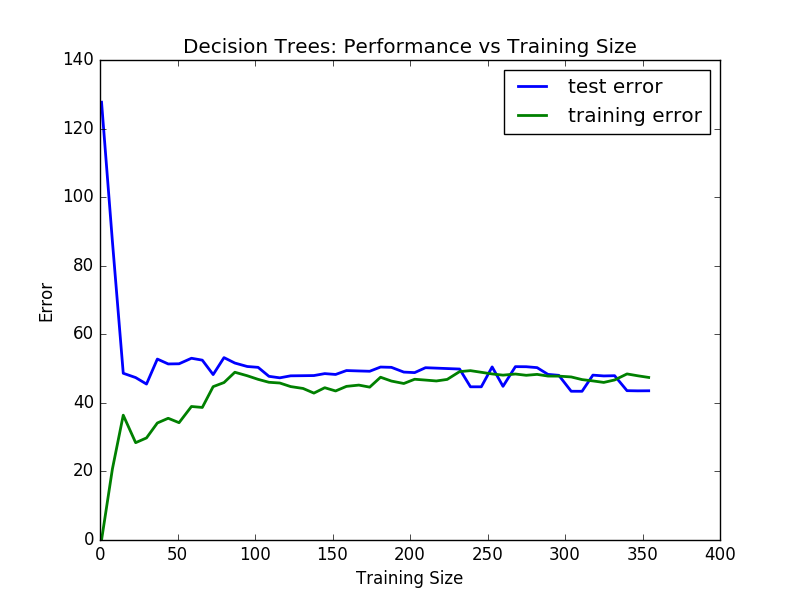
\includegraphics[scale=0.4]{figure_1}
		\caption{Learning curve for max\_depth $= 1$.}
\end{center}
\end{figure}


\newpage

We see that the training and testing error initially converge at a high value, and as we increase the complexity of the model, the training and testing error start to converge at lower values. However, as we keep increasing the complexity, the testing error stays roughly the same (or even becomes slightly worse) while the training error continues to decrease. This is the sign of overfitting. Comparing the first and last learning curves (the learning curves for the decision tree regressor with max depth 1 and 10, respectively) we see that, when fully trained, the first model suffers from high bias (the error is high as the model is not complex enough to accurately model the data) while the last model suffers from high variance (it is too complex - by overfitting the training data, it is not predictive of the testing data). 

\begin{figure}[h]
\begin{center}
		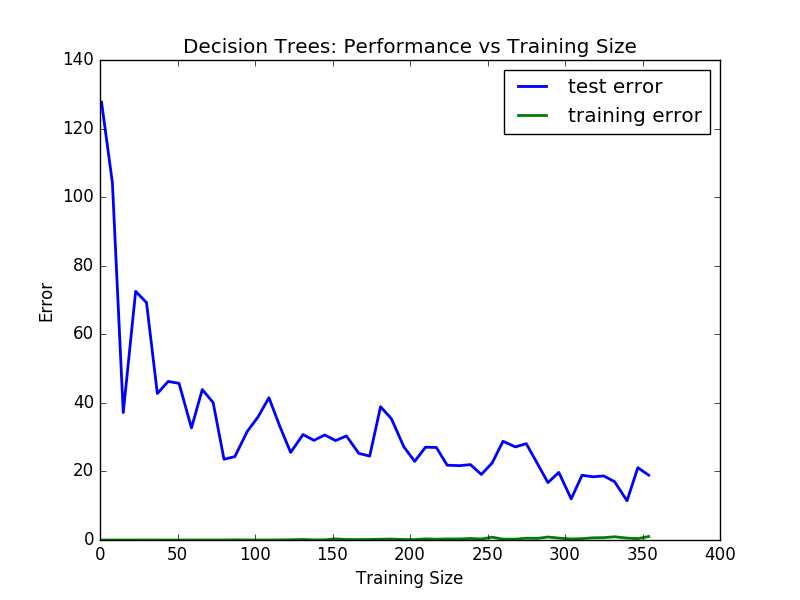
\includegraphics[scale=0.4]{figure_10}
		\caption{Learning curve for max\_depth $= 10$.}
\end{center}
\end{figure}

\newpage

We can visualize this by plotting a \emph{model complexity graph}, which plots the training and testing error of each fully trained model against the max depth of the decision tree regressor. This is implemented by the following code:

\begin{verbatim}
	def model_complexity(X_train, y_train, X_test, y_test):
    """Calculate the performance of the model as model complexity increases."""

    print "Model Complexity: "

    # We will vary the depth of decision trees from 2 to 25
    max_depth = np.arange(1, 25)
    train_err = np.zeros(len(max_depth))
    test_err = np.zeros(len(max_depth))

    for i, d in enumerate(max_depth):
        # Setup a Decision Tree Regressor so that it learns a tree with depth d
        regressor = DecisionTreeRegressor(max_depth=d)

        # Fit the learner to the training data
        regressor.fit(X_train, y_train)

        # Find the performance on the training set
        train_err[i] = performance_metric(y_train, regressor.predict(X_train))

        # Find the performance on the testing set
        test_err[i] = performance_metric(y_test, regressor.predict(X_test))

    # Plot the model complexity graph
    model_complexity_graph(max_depth, train_err, test_err)


def model_complexity_graph(max_depth, train_err, test_err):
    """Plot training and test error as a function of the depth of the decision tree learn."""

    pl.figure()
    pl.title('Decision Trees: Performance vs Max Depth')
    pl.plot(max_depth, test_err, lw=2, label = 'test error')
    pl.plot(max_depth, train_err, lw=2, label = 'training error')
    pl.legend()
    pl.xlabel('Max Depth')
    pl.ylabel('Error')
    pl.show()
\end{verbatim}

\begin{figure}[t]
\begin{center}
		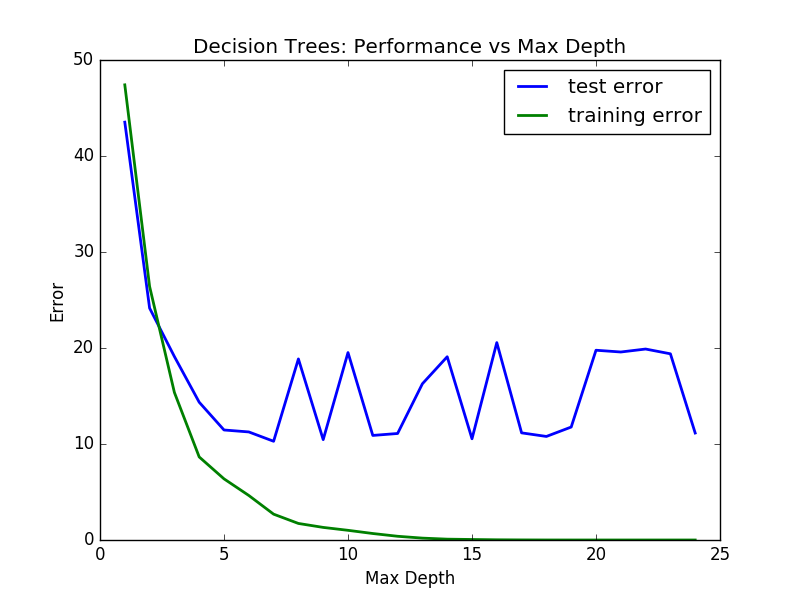
\includegraphics[scale=0.4]{model_complexity}
		\caption{Model complexity graph.}
\end{center}
\end{figure}

Looking at the graph, we can confirm that training and testing errors initially decrease together as we increase model complexity, until the testing error levels off (although fluctuating) and the training error continues to decrease. The region where these two errors diverge is the overfitting region, so we can read off from the graph that a max depth of 4 best generalizes the dataset.

\newpage

\subsection{Model Prediction}
After implementing \texttt{GridSearch} as above, we print \texttt{clf.best\_estimator\_} to see the best model. Due to the small randomization in the code where we split the dataset into training and testing sets, we run the program several times to identify the most common optimal model complexity, which leads to the most reasonable price. As we determined visually above, the best model is given by 

\begin{verbatim}
	>>> clf.best_estimator_
DecisionTreeRegressor(criterion='mse', max_depth=4, max_features=None,
           max_leaf_nodes=None, min_samples_leaf=1, min_samples_split=2,
           min_weight_fraction_leaf=0.0, presort=False, random_state=None,
           splitter='best')
\end{verbatim}
For our example house, the price predicted by this model is 
\begin{verbatim}
	>>> x = [11.95, 0.00, 18.100, 0, 0.6590, 5.6090, 90.00, 1.385, 24, 680.0,
	    ... 20.20, 332.09, 12.13]	
>>> y = clf.best_estimator_.predict(x)
>>> print "Prediction: " + str(y)
Prediction: [ 21.62974359]
    
\end{verbatim}
Comparing with the statistics computed in section \ref{stats}, this price is well within one standard deviation of the mean, and very close to the median price.



\section{Conclusions}\label{conclusions}
In this project, we have used a decision tree regressor to model housing prices using the Boston housing dataset. By implementing a grid search over maximum tree depths, we found that the optimal model has a maximum depth of 4. We then used this model to predict the price of a new house, which is not included in the dataset. By comparing our prediction with the statistics computed from the dataset, we find that our prediction is reasonable.

Due to the small randomization in the code that splits our data into a training and testing set, we needed to run our program several times to find the most common optimal model and predicted price. This might be improved by increasing the number of foldings from the default 3-fold cross validation used by grid search. However, this would come at the cost of longer computation time, and for the purposes of this project the method employed here produces a satisfactory answer.
\end{document}